%% GENERATED by tools/from_docs.py from stepss-docs. Do not edit by hand:
%% edit the page named below in stepss-docs and regenerate.
%% source: stepss-docs/src/content/docs/gui/first-run.mdx

\chapter{First run of STEPSS GUI}\label{doc:gui-first-run}

STEPSS GUI is the desktop edition: the one an installer puts on your machine, and
the one that carries every engine plus CODEGEN. This page covers the first launch
and gets you to a working simulation without you supplying any data of your own.

If it is not installed yet, start at
\hyperref[ch-install]{Installing STEPSS GUI}.

\section{Accepting the licence}\label{gui-first-run:accepting-the-licence}

The first launch shows a licence and will not continue until you accept it.

The licence on that screen is \textbf{RAMSES's}, not the interface's. The two user
interfaces are Apache 2.0, while the dynamic simulator is the property of the
University of Li\`ege and free for non-commercial use only, so the dialog names the
component rather than the application. The free version is also capped, in ways
worth knowing before you build a large case.

\hyperref[ch-legal]{License} is the one page that states the terms, the
caps and which component each applies to. Read it there rather than inferring
them from the dialog.

\begin{figure}[htbp]
\centering

\includegraphics[width=0.98\linewidth]{figures/gui-license-light}
\caption{The License Agreement dialog on first launch.}
\end{figure}

You accept once. Later launches go straight to the window.

\section{Start from a bundled example}\label{gui-first-run:start-from-a-bundled-example}

The fastest way to see STEPSS work is not to load anything of your own. The
application ships four complete test systems, and opening one copies it to disk
and fills in every file slot, so \textbf{Run} works immediately.

\begin{enumerate}
\def\labelenumi{\arabic{enumi}.}
\item
  Open the \textbf{File} menu.
\item
  Choose \textbf{Open Examples}.
\item
  Pick a system from the list. The panel beside it describes the case, its size
  and what the shipped disturbance does.
\item
  Click \textbf{Open example}.
\end{enumerate}

\begin{figure}[htbp]
\centering
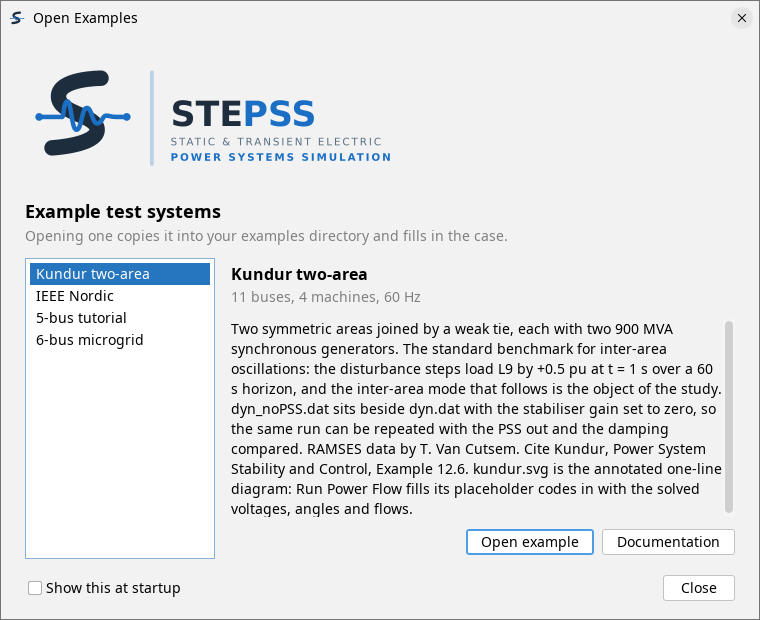
\includegraphics[width=0.98\linewidth]{figures/gui-open-examples-light}
\caption{The Open Examples dialog.}
\end{figure}

A banner across the top of the window then reports where the copy landed, with an
\textbf{Open folder} button to reveal it, and \textbf{Dismiss} to put it away. Behind it
every file slot is already filled in.

\begin{figure}[htbp]
\centering
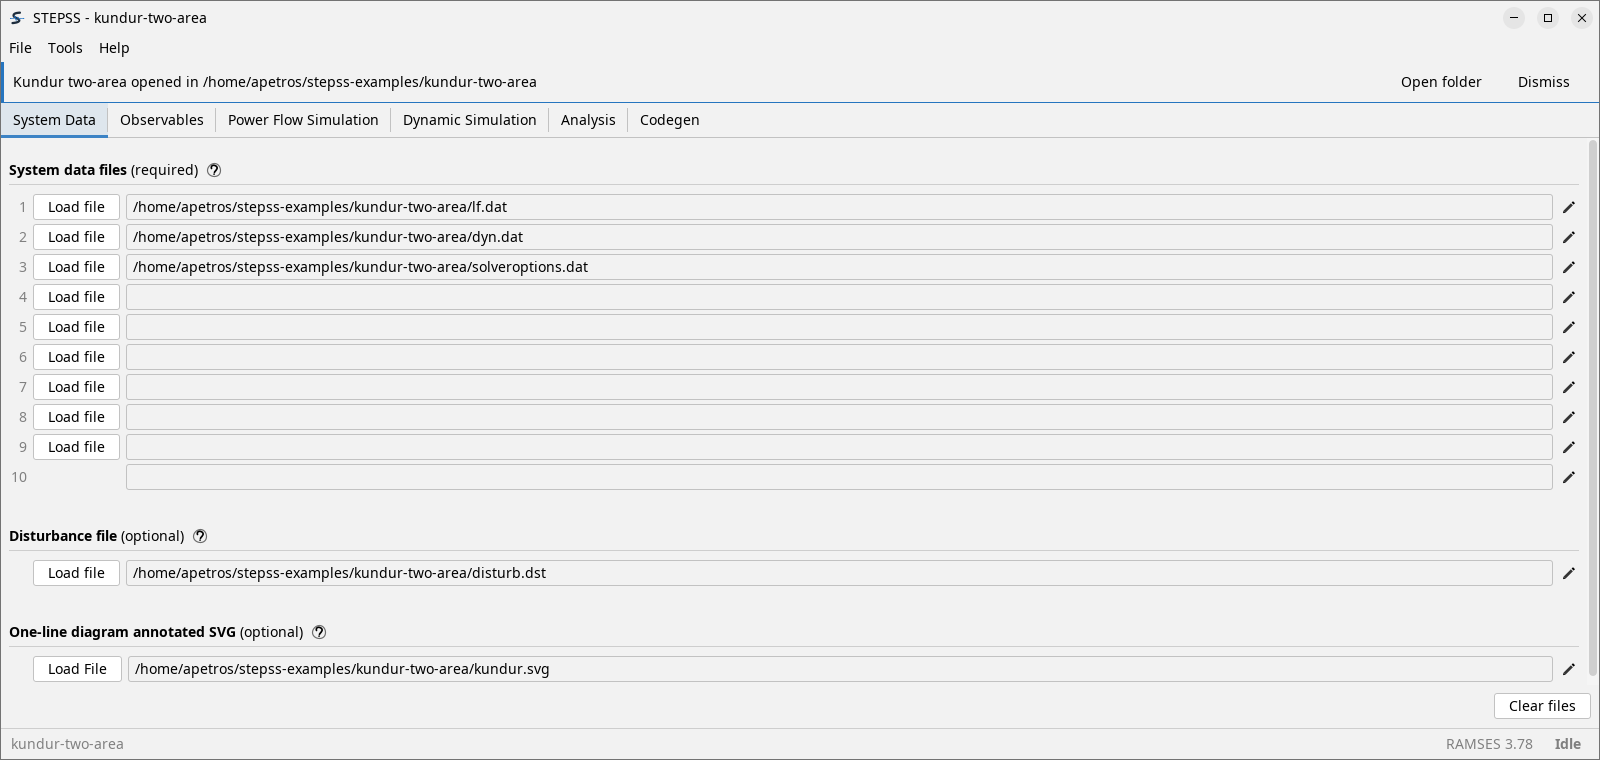
\includegraphics[width=0.98\linewidth]{figures/gui-example-banner-light}
\caption{The System Data tab immediately after opening the Kundur two-area example.}
\end{figure}

The dialog appears on startup by default. Clear \textbf{Show this at startup} to stop
that, and reach it from \textbf{File, Open Examples} whenever you want it back.

\section{The four bundled systems}\label{gui-first-run:the-four-bundled-systems}

{\def\LTcaptype{none} % do not increment counter
\begin{small}\begin{longtable}[]{@{}
  >{\raggedright\arraybackslash}p{(\linewidth - 4\tabcolsep) * \real{0.3333}}
  >{\raggedright\arraybackslash}p{(\linewidth - 4\tabcolsep) * \real{0.3333}}
  >{\raggedright\arraybackslash}p{(\linewidth - 4\tabcolsep) * \real{0.3333}}@{}}
\toprule\noalign{}
\begin{minipage}[b]{\linewidth}\raggedright
System
\end{minipage} & \begin{minipage}[b]{\linewidth}\raggedright
Size
\end{minipage} & \begin{minipage}[b]{\linewidth}\raggedright
What it is for
\end{minipage} \\
\midrule\noalign{}
\endhead
\bottomrule\noalign{}
\endlastfoot
\hyperref[doc:ts-5bus]{5-bus tutorial} & 5 buses, 1 machine & The teaching case from EEN452 at the Cyprus University of Technology, and the one to open first. One generator with detailed machine, governor and AVR models, a composite load, and an external grid, small enough to read end to end. Its disturbance file is deliberately empty, ready for you to add the records of the study you want. \\
\hyperref[doc:ts-kundur]{Kundur two-area} & 11 buses, 4 machines, 60 Hz & The standard benchmark for inter-area oscillations. Two symmetric areas joined by a weak tie. The shipped disturbance steps a load and the resulting inter-area mode is the object of the study. A second dynamic file with the stabiliser disabled ships beside the first, so the same run can be repeated with the PSS out and the damping compared. \\
\hyperref[doc:ts-nordic]{IEEE Nordic} & 74 buses, 20 machines, 400/220/130 kV & The reference system for long-term voltage stability, from IEEE PES technical report PES-TR19. It opens on the tripped-branch case it is best known for, with further disturbances, a second operating point and a set of load-increase variants shipped alongside. \\
6-bus microgrid & 6 buses, 2 generators, 6/11 kV & A power-flow-only case: two lines, four transformers, loads at buses D and E, and generators at A (slack) and F. It carries no dynamic data and no disturbance scenario, so it runs on \textbf{Power Flow Simulation} and not on \textbf{Dynamic Simulation}. It is the case the \hyperref[ch-pf]{annotated one-line diagram} is demonstrated with: \texttt{6bus.svg} is a template of placeholder codes that \textbf{Run power flow} fills in with the solved values. \\
\end{longtable}\end{small}
}

The first three link to their own page here, which carries the network, the
models and the studies the system is used for; the microgrid has no page of its
own, because everything it demonstrates belongs to
\hyperref[ch-pf]{Power Flow}. \textbf{Documentation} in the dialog opens the
system's source repository in every case.

\section{Where the files go}\label{gui-first-run:where-the-files-go}

Two directories are remembered separately, and the distinction matters once you
open more than one example.

\begin{itemize}
\tightlist
\item
  The \textbf{examples directory} is where copies are unpacked. Opening a second
  example puts it beside the first rather than inside it.
\item
  The \textbf{working directory} is where a run reads and writes. Opening an example
  moves it into that example.
\end{itemize}

Set either from the \textbf{Tools} menu, which also offers \textbf{Open working folder} and
\textbf{Open terminal in working folder} for getting at the files directly.

An example is copied rather than run in place, so editing it is safe and the
copy survives quitting. That is the point of copying: work on it freely.

\section{Real-time plotting}\label{gui-first-run:real-time-plotting}

STEPSS GUI plots curves while a simulation runs, which is covered on
\hyperref[doc:gui-interface]{The Interface}. It draws them itself: nothing has to be
installed on any platform, and no external plotting program is involved.

Each runtime observable you filled in gets a panel of its own, stacked on a
shared time axis, and the window keeps drawing until the run ends. \textbf{Save
PNG} and \textbf{Save CSV} keep the picture or the samples behind it, and \textbf{Reset
zoom} returns to the full horizon after a drag.

\begin{figure}[htbp]
\centering
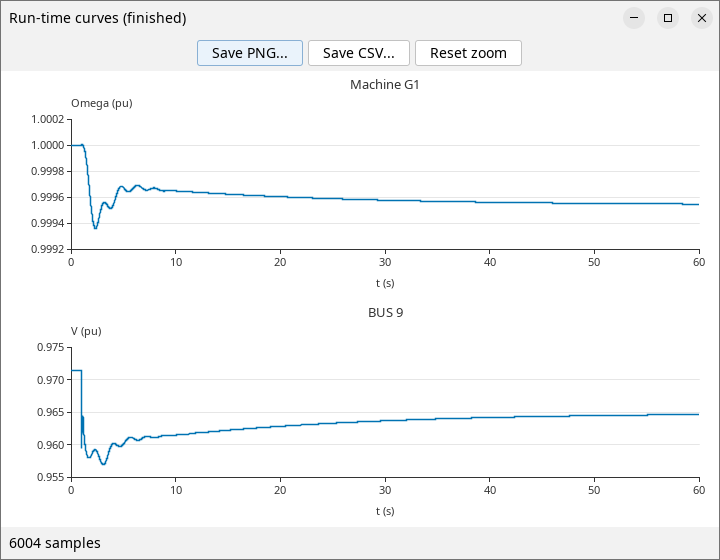
\includegraphics[width=0.98\linewidth]{figures/gui-runtime-curves-light}
\caption{The Run-time curves window at the end of a Kundur run, titled Run-time curves (finished).}
\end{figure}

Run-time curves need a RAMSES release that writes a column map into the header
of its observable file. Against an engine that does not, the window says so
rather than drawing. Extracting curves after a run is independent of this: that
path reads DYNGRAPH's output, which carries no header.

\begin{docsnote}{Could not prepare the simulation toolchain}

The engines ship inside the application and are unpacked to a temporary
directory each time it starts. A \textbf{Toolchain error} on launch means that
unpacking failed, almost always because the temporary directory is not
writable. Fix that and start again.

\end{docsnote}

\section{Choosing a theme}\label{gui-first-run:choosing-a-theme}

\textbf{Tools}, then \textbf{Dark theme}. The choice is remembered between sessions, along
with the window's size and position.

\section{Next steps}\label{gui-first-run:next-steps}

\begin{itemize}
\tightlist
\item
  \hyperref[doc:gui-interface]{The Interface}, what each tab is for
\item
  \hyperref[doc:gui-running]{Running a Simulation}, a complete run on the Kundur case
\item
  \hyperref[ch-files]{File Formats}, what goes in the files you loaded
\end{itemize}
